 % -*- root: ../medieninformatik-arbeit.tex -*-
\documentclass[../medieninformatik-arbeit.tex]{subfiles}
\begin{document}
\section{Implementation}
\label{ch:configurator}
The implementation of the activity sculpture configurator and the activity sculpture were undertaken in a period of around two months. The developed web configurator in this work makes use of cutting edge technologies for both web development and 3D visualization. This project is a demonstration of the capabilities of current web technologies that allow the developing of fully functional data visualization systems that offer integration with other web services for data interchange and support real time interactive 3D visualization.

This chapter will discuss all aspects of the technical implementation of the prototypes discussed in chapter \ref{ch:proto}. The technical requirements for the system will be discussed in the first section followed by an overview of the used technologies. Further on the modules conforming the system and their relationship will be explained in the architecture section. THe configurator section covers the implementation of the controls used by the user to manipulate the sculpture and the generation of the sculpture which are the main functionalities covered in the front end side of the application. The integration of the Whithings API and the manipulation performed on the received data are covered in the backend section of the chapter. Finally an overview of the challenges encountered while developing the system is presented. 

\subsection{Requirements}
Through the analysis of current works described in chapter \ref{ch:related},the requirements of the prototypes in chapter \ref{ch:proto} and in view of the forthcoming user study the functionality and technical requirements of the web-based activity sculpture creator were formulated as follows.

\begin{itemize}
	\item Implement the designed configurator workflow views
	\item Users have to be able to login with their personal Withings account
	\item Query user's data with the Withings API
	\item Store user's data and profile information in a data base
	\item Implement user interface control widgets like buttons, sliders and toggles for the customization area of the configurator
	\item Implement the designed activity sculpture geometry
	\item The visualization of the sculpture has to be rendered in real time  
	\item Changes made in the configurator have to be reflected in the sculpture instantly. avoid the use of update buttons 
	\item Users have to be able to navigate the sculpture in 3D space through rotation and zooming interactions
	\item STL file export support for 3D printing
	\item Support for current browsers
	\item Deployment of a fully working version in a web server for the general public. Anybody with a Withings account should be able to use it an visualize their data.
\end{itemize}


The required functionality is beyond what it would be needed for a basic working prototype. The developed configurator in this work is a fully functional system that fulfills every requirement specified in this section. The stated requirements involved the implementation of other functionality to ensure the requirement was fulfilled. For example the login functionality implies the implementation of an Oauth authentication solution(explained later in section \ref{sub:ApiIntegration}) in order to integrate with the Withings API. Also because the configurator is dealing with personal data the security of the system is important, as a basic approach to address this, the configurator implements session handling.

In the following section the used technologies to tackle the extensive list of requirements will be presented.  

\subsection{Technology}
The web configurator was developed with a modern stack of technologies that enable the use of the JavaScript language not only for frontend but also for the backend, the database and graphics programming. The MEAN stack is a collection of technologies that enables developers to write web applications in a single programming language. MEAN is the acronym for the technologies  conforming the stack: \textit{MongoDB}\cite{mongodb}, \textit{Express}\cite{express}, \textit{AngularJS}\cite{angular} and \textit{Node.js}\cite{joyent2015node}. The acronym was first used by Valeri Karpov, MongoDB engineer, in a blog post\cite{meanstack} where he discussed the benefits of using the same language across all technologies involved. Among the benefits Karpov states their team have experienced an increment in the performance of the developed software and also in the team's productivity. In short the MEAN stack's frameworks will be introduced. 

\textbf{MongoDB} is an ``open-source, document database designed for ease of development and scaling''\cite{mongodb}. Document based are conformed of collections (the equivalent of tables) which can contain several documents (rows) that  to any schema are in essence JSON Objects (JavaScript Object Notation). MongoDB does not enforce any schema to the stored data, making it a very flexible environment to work with. In MongoDB queries are performed in JavaScript providing a seamless integration of the JavaScript language, from querying the information to structuring it in JSON objects. The stored JSON objects are encoded to the BSON format which stands for Binary JSON to enhance efficiency and provide additional data types. Even though working with a schema-less database brings great flexibility, it is recommendable to bring some consistency to the MongoDB documents. For this purpose an object modeling library called \textit{mongoose}\cite{mongoose} has found broad adoption in the developer community. Mongoose provides functionality to easily model the application's data with type casting, custom query functions and other niceties. To illustrate how a mongoose schema looks like, listing \ref{list:mongoose-schema} shows an excerpt of the user schema designed for the configurator.

\begin{lstlisting}[style=htmlcssjs, caption={An excerpt of the user mongoose schema},label=list:mongoose-schema]
// load the mongoose module
var mongoose = require('mongoose');
var Schema = mongoose.Schema;

var userSchema = new Schema({
  profile: {
    name: String, //data type definition
    gender: Number,
    age: Number,
    location: String
  },
// more fields... 
  settings: {
    startDate: Date,
    endDate: Date,
    show: Boolean
  },
  sculptures: {type: Array, "default": []}
});
\end{lstlisting} 

\textbf{Node.js}\cite{joyent2015node} and \textbf{Express}\cite{express} are the frameworks used to develop the web server of the application. Node.js is backend JavaScript, based on the ``V8'' chrome JavaScript runtime providing an event-driven architecture and non-blocking i/o allowing for high performance real time applications. \textit{Node.js} is conformed of basic modules that provide network functionality but it requires the developer to build everything from the ground up. To address this issue the JavaScript library \textit{Express} was developed. Express provides a rich set of features like routing, middleware support and HTTP utilities that allow rapid development of network applications. Listing \ref{list:node-server} shows how a simple server is implemented with Node.js and Express.

\begin{lstlisting}[style=htmlcssjs, caption={Basic Node.js and Express server example},label=list:node-server]
var express = require('express');
var app = express();

app.get('/', function (req, res) {
  res.send('Hello World!');
});

var server = app.listen(3000, function () {
  var host = server.address().address;
  var port = server.address().port;
  console.log('Example app listening at http://%s:%s', host, port);
});
\end{lstlisting}

\textbf{AngularJS}\cite{angular} is the fronted framework in the MEAN stack. \textit{AngularJS} is an opens-source project developed by Google for the development of Single Page Applications (SPAs) where the whole content of a web page is rendered in a single web page and the content is either completely loaded at the beginning or its injected according to user interactions. AngularJS is based on a Model-View-Whatever design pattern (MVW) that allows developers to choose the design pattern that better accommodates their coding style. Whichever design pattern is chosen, AngularJS enforces developers to structure code into modules providing a strong organization in the code base. The functionality provided by AngularJS ranges from bidirectional data-binding, routing, form validation, server communication tools and directives that allow the creation of custom HTML syntax. With frameworks like AngularJS SPA allow to take much of the server workload to the frontend. Another feature of AngularJS is its extensibility. For the purposes of this work the \textit{Angular Material}\cite{angularmaterial} was utilized to implement user interface controls and theming. The \textit{Angular-Material} module is also developed by Google and it provides a solid framework for developing user interfaces utilizing the ``Material design'' philosophies. 

The graphic visualization of the sculpture was implemented with the \textit{Threejs}\cite{cabello2010three} library which provides an approachable abstraction of the \textit{WebGL} API. WebGL is a standard that provides hardware accelerated 3D graphics rendering for the web\cite{webgl}. Based on the OpenGL ES 2.0 standard, WebGL allows the development of real time visualizations in JavaScript through the use of the HTML 5 canvas element. \textit{Threejs} offers developer a wide set of tools and abstractions for rapid development of graphic applications in the web. An example of a basic Threejs application is composed of a scene object that contains cameras, lights and mesh objects that will be rendered to the canvas through a WebGL context. Listing \ref{list:threejs-app} provides a basic example of setting up a the renderer and attaching it to the DOM, loading cameras and lights, creating the scene, adding a cube mesh and finally rendering it.

\begin{lstlisting}[style=htmlcssjs, caption={Basic Threejs 3D app example},label=list:threejs-app, float=t]
var camera, scene, renderer;
var geometry, material, mesh;

renderer = new THREE.WebGLRenderer();
renderer.setSize( window.innerWidth, window.innerHeight );
document.body.appendChild( renderer.domElement );

camera = new THREE.PerspectiveCamera( 50, window.innerWidth/window.innerHeight, 1, 10000 );
camera.position.z = 500;

scene = new THREE.Scene();
					
geometry = new THREE.CubeGeometry(200, 200, 200);
material = new THREE.MeshNormalMaterial({shading: THREE.FlatShading});
mesh = new THREE.Mesh(geometry, material);

scene.add( mesh );
renderer.render( scene, camera );
\end{lstlisting}

In the following sections the utilization the benefits of developing with the MEAN stack with other technologies will be highlighted through examples of modules developed for the web configurator. 

\subsection{Architecture}
By using the MEAN stack to develop the web configurator certain architecture decisions are enforced. One being the use of the backend more as a RESTFul web API (Representational State Transfer) for querying data than for requesting the generation of pages. RESTful APIs define a modern architectural model over the HTTP protocol to perform service operations over a system's data\cite{Fielding:2000:PDM:337180.337228}. A great advantage of utilizing RESTful architectures is that it provides good scalability as the backend can be completely decoupled from the client implementation, meaning one backend can be used to provide data to all sorts of clients from web clients to mobile or desktop applications. The configurator's backend is composed of a web service that implements the Withings API for authentication and requesting sensor data, session handling for assuring only logged in users can access the configurator's backend, the user data API that interacts with the MongoDB database to perform CRUD (Create, Read, Update, Delete) operations on the gathered user data and WebSocket communication support. WebSocket is a protocol based on a TCP connection that provides full-duplex communication to client-server applications\cite{fette2011websocket}. The advantage of WebSockets is that it allows servers to push data to clients without being requested. The configurator makes use of WebSockets through the \textit{Socket.io}\cite{socketio} library which implements the use of WebSockets in an event-driven pattern. Third party libraries utilized in the backend are contained in Node.js modules. Figure \ref{fig:architecture} provides an overview of the modules conforming the backend and frontend sides of the configurator.  

\begin{figure}[h]
\captionsetup{width=\textwidth}
\begin{center}
  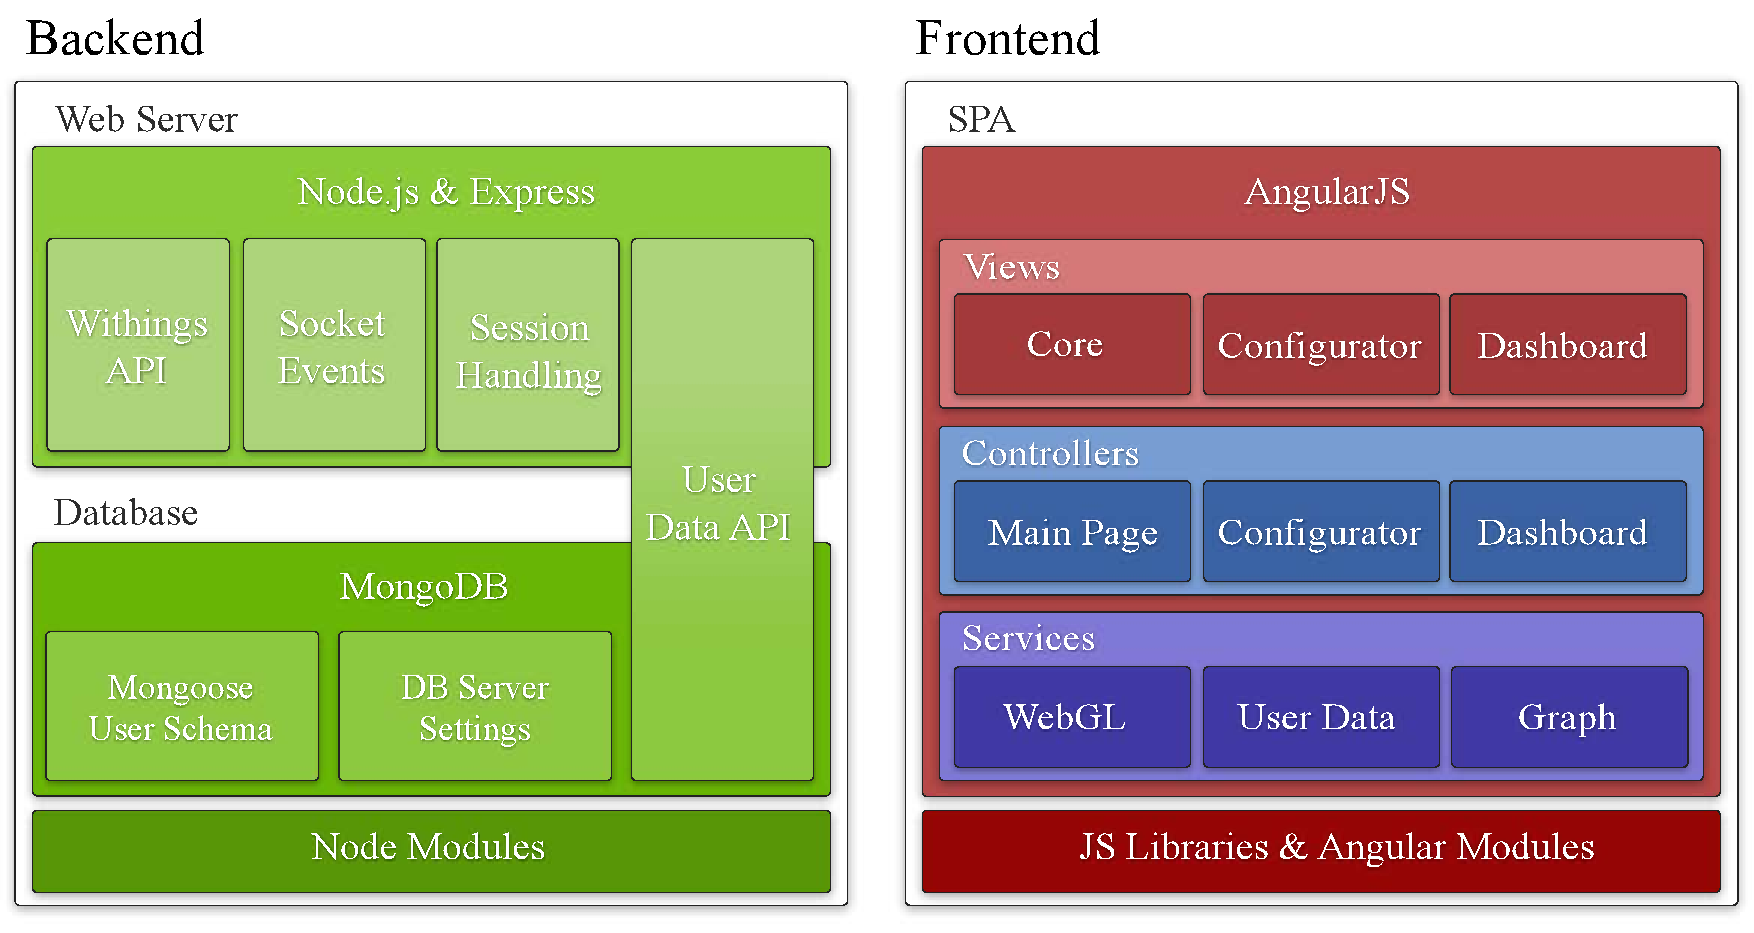
\includegraphics[width=\textwidth]{Configurator/img/Architecture}
  \caption{Activity Sculpture web configurator's architecture}
\label{fig:architecture}
\end{center}
\end{figure}

The frontend of the configurator is a SPA implemented in AngularJS. As discussed before, the backend is implemented as a Web API, relegating the generation of the HTML content to the AngularJS application. The frontend implementation follows a Model View Controller (MVC) pattern for better separation of concerns. Due to the flexibility of AngularJS this is was implemented through the extensive use of controllers attached to views. In AngularJS views are basic HTML templates that describe the visual aspect of the web site. Controllers implement logic functionality to manipulate the application's data or model. The model part of the MVC pattern is implemented by Angular services. Services in Angular are modules that can interface with databases through web APIs or they can be used to abstract functionality and reuse it across the application. Views can host several controllers who at the same time can access several services. 

Even though views in the configurator are divided in several parts for re-usability across the application, they were separated in three main areas: the core, the configurator and the dashboard. The core comprehends partial views utilized for the welcome page, the consent window and the 404 error page. The configurator's view contains several modules with User Interface (UI) controls and the canvas for the sculpture. The dashboard view is composed of the dashboard view that shows the sculpture gallery and charts visualizing the user's data, and the setup form. 

The attached controllers to these views provide the logic to achieve the intention of each section. Due to the specific requirements of each section in the configurator, the controllers are also organized in modules for the main page, the configurator and the dashboard. The main page controller provides the logic for starting the authentication process. The configurator controller is the most complex as it implements the logic the UI controls and the rendering of the sculpture. The configurator controller makes heavy use of the graphics service module, which manages Threejs scenes, cameras and the generation of the sculpture. Further more the configurator controller reaches to the user data service to load the data for the generation of the sculpture. The user data service contains several modules for data manipulation and transforming and provides a user object that holds all the data received from the Withings API. The user object follows a singleton pattern implementation, making a single instance of the object available throughout the application. This is specially helpful as the dashboard configurator also needs the data provided by the user object in order to visualize generate the charts and load the sculpture gallery. For the generation of charts the dashboard controller makes use of a graph service that implements a JavaScript SVG library called \textit{D3.js}\cite{bostock2015d3js}, which stands for ``Data driven documents''. The \textit{D3.js} library has gained broad popularity in web data visualization as it provides great flexibility through data-driven DOM manipulation and the use of widely supported CSS, SVG and JavaScript technologies. 

An important part of every AngularJS application is the mapping of views and controllers to routes. In SPAs the rendering of websites is performed client side and not requested from the backend as in other architectures. In order to achieve this the application defines routes that are in essence URL addresses that represent a certain part of the application. When a route is called the application maps the address to a view with controllers presenting to the user the requested site. AngularJS provides a routing module but for this work a third party angular module called UI-Router was utilized. The UI-Router framework developed by the Angular-UI team\cite{ui-router} provides routing functionality by organizing views into a state machine, unlike AngularJS that is based on URLs. Every state can have a controller and a view with child views assigned to it, it is not strictly necessary to map a state to a URL but it can be done. Added to that states can contain nested stated states for complex routing implementations. 

Other secondary functionality is implemented through the use of JavaScript libraries and angular modules. 

In order to better illustrate how the different parts of the application interact with each other a flow diagram of the application can be seen in figure \ref{fig:flowdiagram1} and \ref{fig:flowdiagram2}. The flow diagram explains in a simplified way the tasks the client, the server, the Withings API and the database perform and the actions the user can perform. The diagram also offers information as of which steps are involved in each of the parts of the application going from the very start where the user starts the configurator in the browser, going over the authentication process, setting up user configurations, presenting the dashboard and finally the configuration process. In upcoming sections some of the most important steps are going to be explained more in depth.

\begin{figure}[hb!]
\captionsetup{width=\textwidth}
\begin{center}
  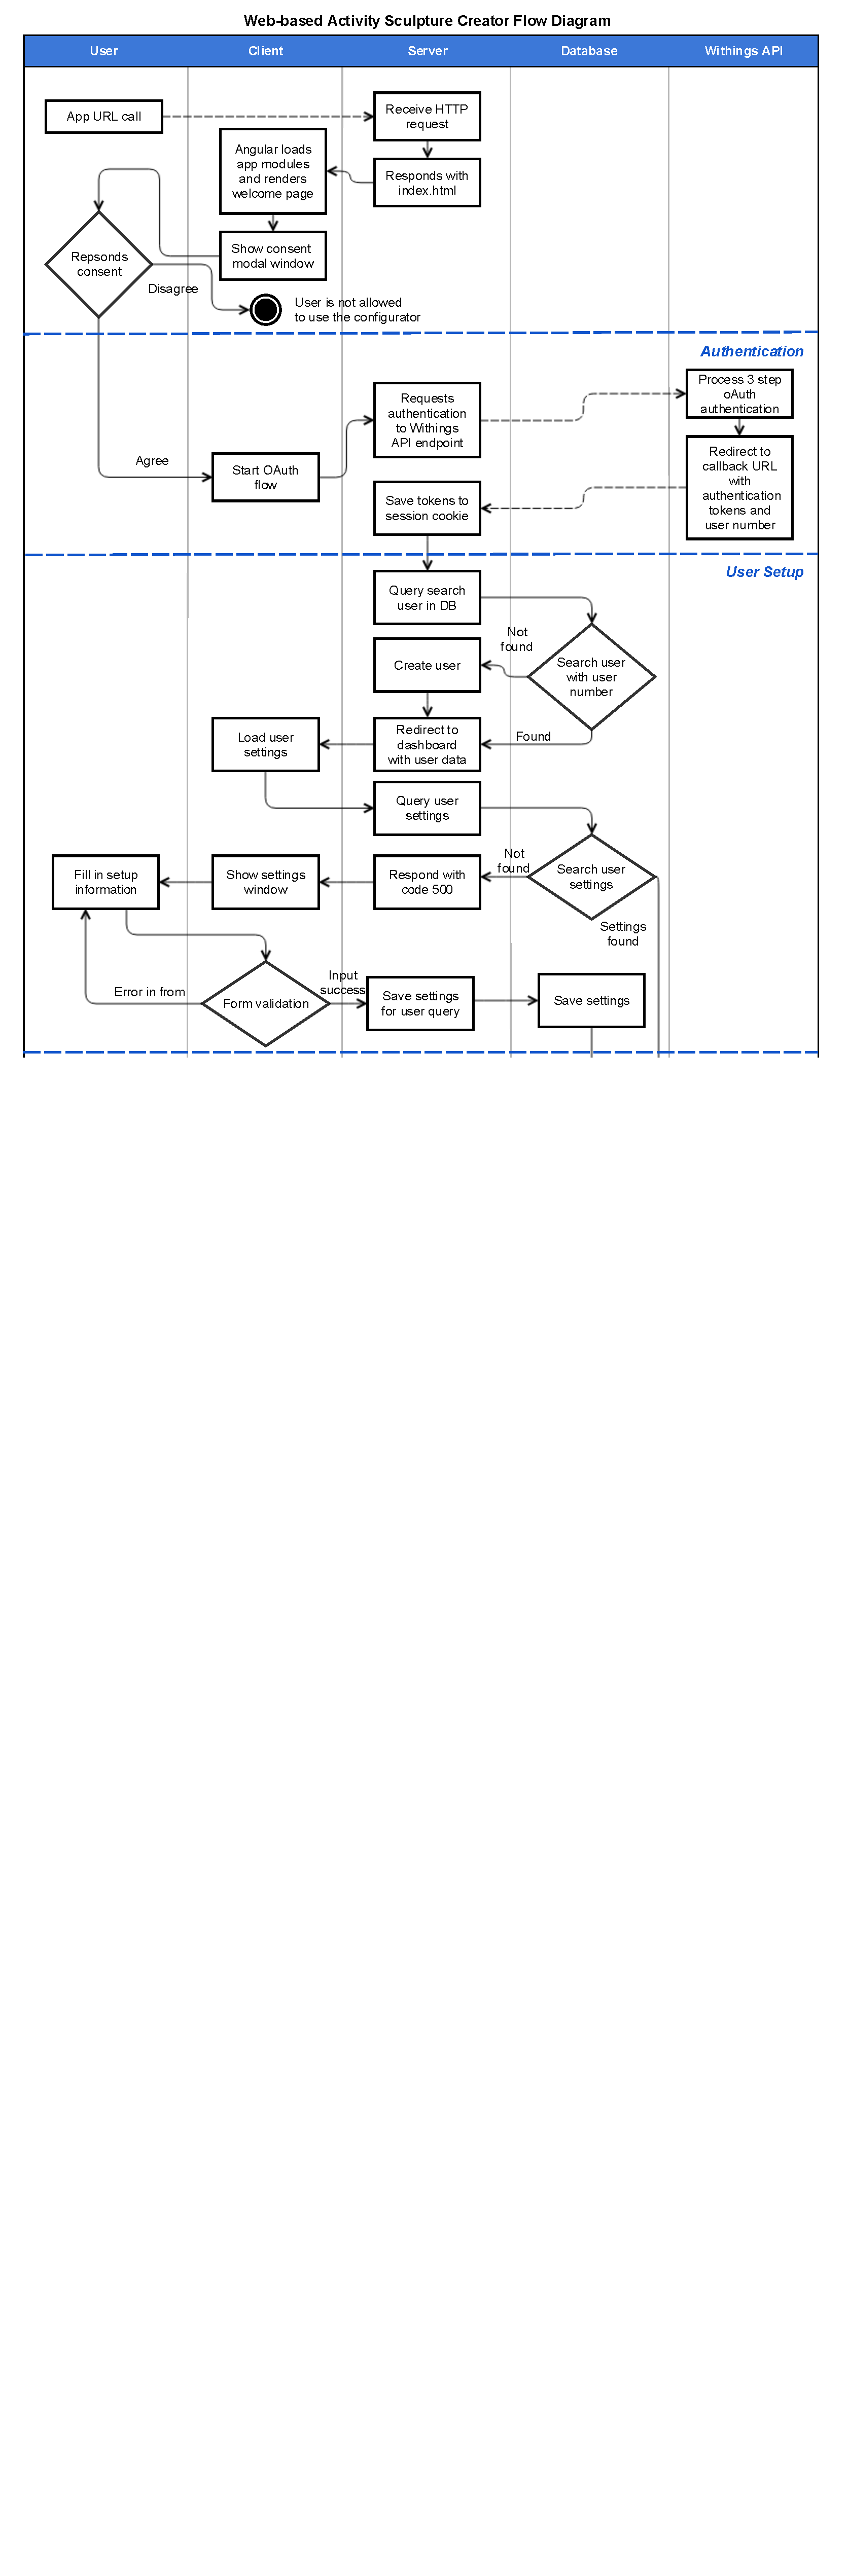
\includegraphics[width=0.82\textwidth]{Configurator/img/flow_diagram_1}
  \caption{Flow diagram part 1}
\label{fig:flowdiagram1}
\end{center}
\end{figure}

\begin{figure}
\captionsetup{width=\textwidth}
\begin{center}
  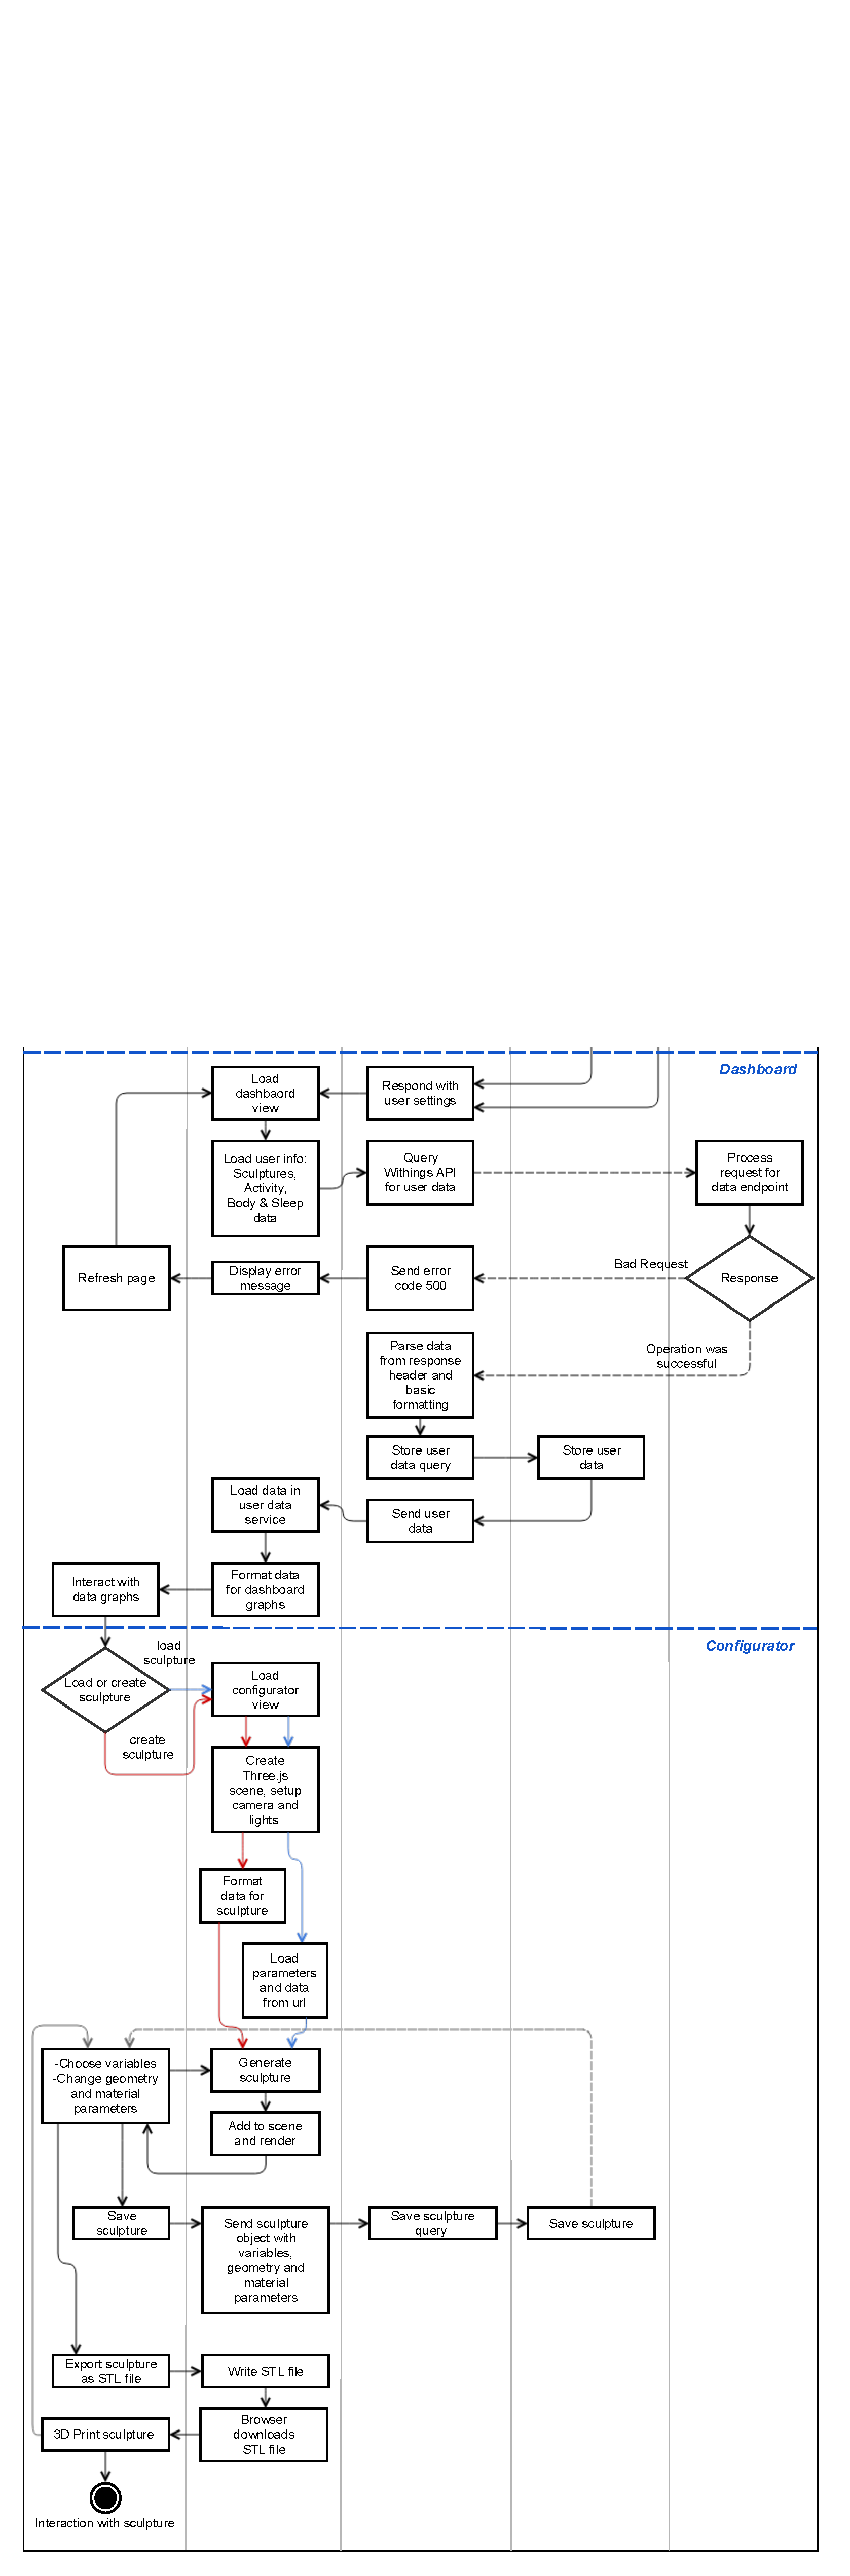
\includegraphics[width=0.82\textwidth]{Configurator/img/flow_diagram_2}
  \caption{Flow diagram part 2}
\label{fig:flowdiagram2}
\end{center}
\end{figure}

\subsection{Configurator}
The configurator section of the activity sculpture creator has two main tasks. The first task being offering users a set of controls for selecting the variables to be mapped into the sculpture and for customizing different aspects of the sculpture. The second task consist in generating the activity sculpture based on the parameters set by the user and rendering it. The steps involved in the execution of both of these tasks are performed by the Angular Application and the interaction of the user (see last section of figure \ref{fig:flowdiagram2}).

\subsubsection{Sculpture Generation \& Rendering}
The generation and rendering of the sculpture is contained in the graphics service module of the application. This service module is composed of 5 submodules: \textit{wcViewport}, \textit{wcScene}, \textit{wcCamera}, \textit{wcModel} and the \textit{WCVaseGeometry} class. 

The \textit{wcScene} is an Angular service that exposes the Threejs scene object. In the same way the \textit{wcCamera} service contains code for configuring the camera and exposing it to the rest of the application. The \textit{wcViewport} submodule is an angular directive, a custom DOM element or attribute attached to an element that extend the element with defined functionality. In the case of the wcViewport it contains setup code for attaching the threejs renderer to the canvas element in the configurator view and it adds the camera from the \textit{wcCamera} service to the \textit{wcScene}  scene object and ultimately renders everything. The \textit{wcModel} service manages the generation of the sculpture by passing the parameters of the UI controllers to the \textit{WCVaseGeometry}, and through the \textit{wcScene} service adds the generated sculpture to the scene object which is rendered every frame. 

The algorithms employed for the generation of the activity vase geometry in the \textit{WCVaseGeometry} class follow the same principles for generating a circular cylinder with equal top and bottom radii. The parameters involved are radius, height and number of height and radial segments. The first two parameters are obvious, radius defines the size of the top and bottom circles and height sets the size in the Y axis. The radial segments define the number of segments that will conform the bottom and top circles. In the same way hight segments are used to define the number of divisions for the sculptures hight. In other words radial and hight segments  With the parameters set, generating the sculpture would require calculating the position vertices of the radial segments for each hight segment. For the activity vase some enhancements were made to this simple principle. As stated in the prototyping phase of the activity sculpture \ref{sub:activtyvase} the idea is to stack radial diagram each with a set of axis representing the activity of one day. In the implementation of \textit{WCVaseGeometry} the radial segments represent the chosen data variables. Each axis will have a different value as the represent different data variables with different magnitudes and units, for example for one day the step count could be 8000 steps and heart-rate 110 bpm. To address this issue all values are normalized to a range that is then added to a ground radius. The hight segments represent the number of days visualized. The algorithm calculates for every day the vertex position of each radial segment from the chosen variables by normalizing the data values and adding that to the base radius. The \textit{WCVaseGeometry} integrates seamlessly with the Threejs. For this in the generation of the sculpture other information had to be generated in order to best integrate with Threejs like calculating vertex and face normals which are needed by some lighting techniques and for mapping textures and materials. Because of the radial diagram concept behind the sculpture does not work well for sculpture visualizing less than 3 variables, further logic had to be implemented in order to always ensure the generation of a 3D sculpture. With one variable the algorithm did not render anything at all, and with two variables the sculpture was a plane with the contours of the axes. This issue was addressed by extruding the same axis over the radius with a predefined number of radial segments. When two variables were chosen, half of the radial segments displayed one variable's values and the second half the other variable's values.  

In order to provide more customization possibilities two more visualization styles were developed. The first is a simple wire-frame visualization that renders only the edges of the faces representing the sculpture. The second style softens each corner's axis by adding more radial segments between each axis, which is achieved through linear interpolation. Figure \ref{fig:sculpture styles} shows the implemented visualization styles for the activity vase. 

\begin{figure}[t!]
\centering
\begin{minipage}{.225\textwidth}
\centering
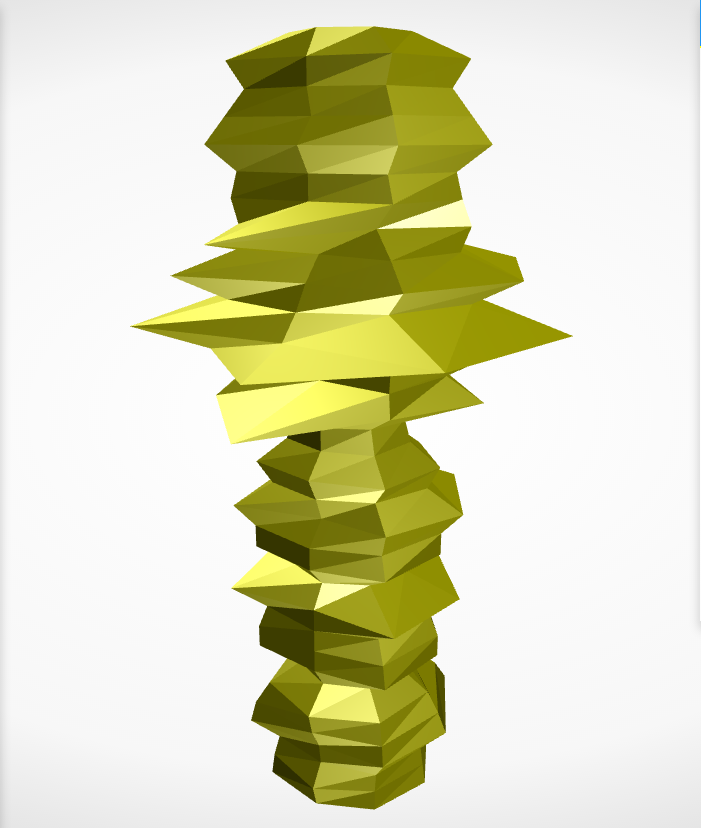
\includegraphics[width=\linewidth]{Configurator/img/sculpture-1}
\end{minipage}
\begin{minipage}{.225\textwidth}
\centering
  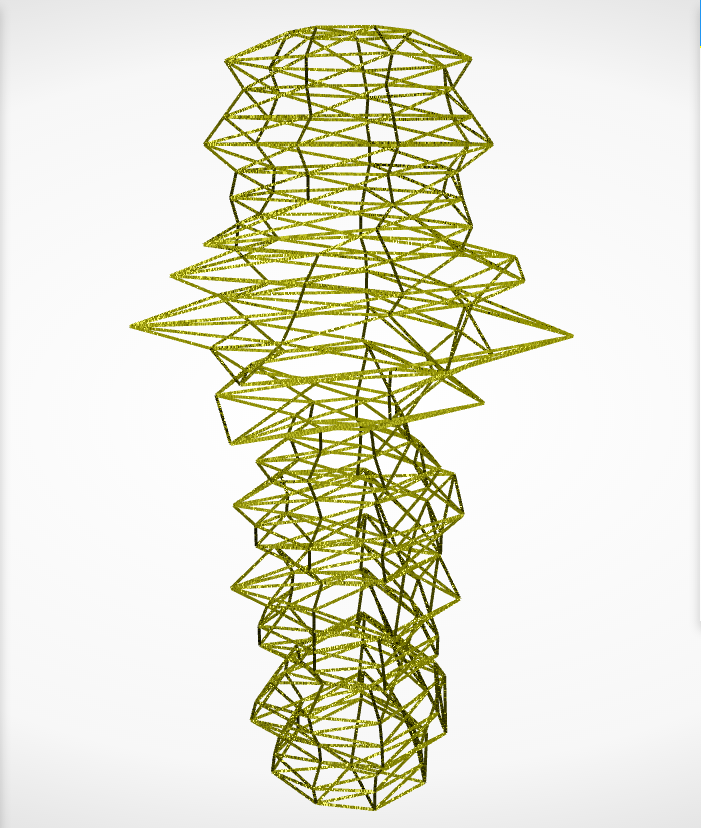
\includegraphics[width=\linewidth]{Configurator/img/sculpture-1w}
\end{minipage}
\begin{minipage}{.225\textwidth}
\centering
  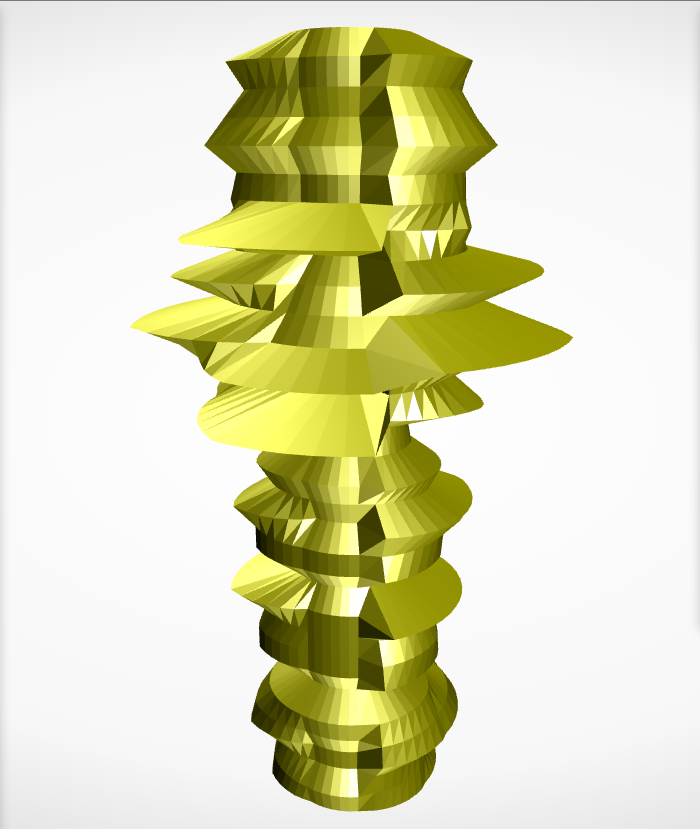
\includegraphics[width=\linewidth]{Configurator/img/sculpture-2}
\end{minipage}
\begin{minipage}{.225\textwidth}
\centering
  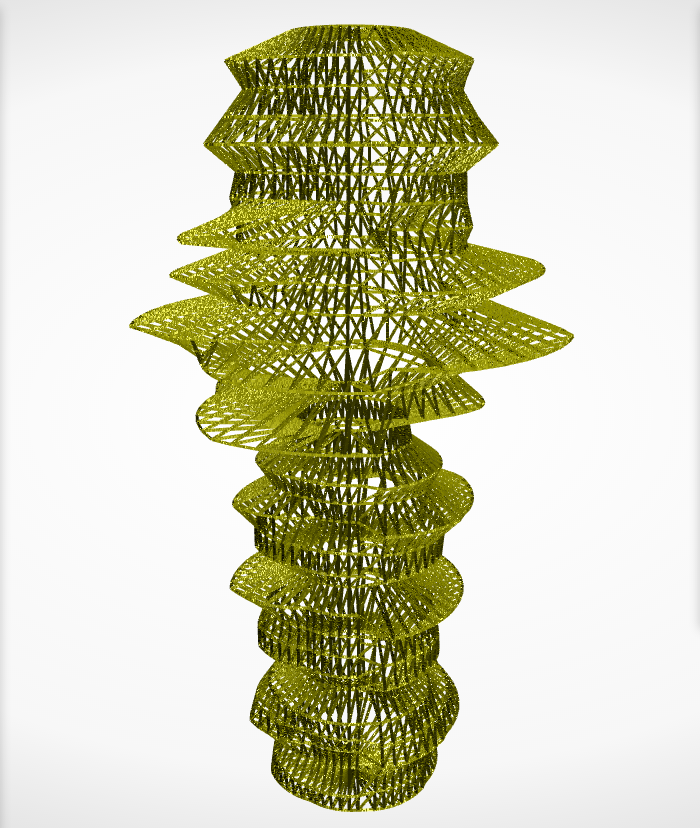
\includegraphics[width=\linewidth]{Configurator/img/sculpture-2w}
\end{minipage}
\caption{\protect Normal and interpolated styles with their wire-frame visualization}
\label{fig:sculpture styles}
\end{figure}

For further technical details regarding the implementation of the activity vase, the complete source code for the \textit{WCVaseGeometry} class can be found in the Appendix \ref{app:source:vasegeometry} of this work.

\subsubsection{Sculpture Manipulation}
\label{sub:sculpturegeneration}
The customization of the sculpture is implemented in the configurator view and its controller who makes use of the graphic and api service modules. When the user calls starts the configurator for creating a sculpture the configurator view loads two panels filled with UI-controls and the \textit{wcViewport} for setting up the visualization engine. 

The customization possibilities are influenced by the design and the implementation of the activity sculpture. The panels displayed by the configurator's view are placed at each side of the screen leaving the sculpture in the middle. The left panel contains two tabs which can be selected for manipulating different parameters. The first tab is the ``Data'' tab and offers an overview of the data variables categorized in activity, body and sleep. Under activity users can choose the from three levels of activity intensity duration namely intense, moderate and soft, elevation, calories burned, distance walked and step count. The body category offers heart pulse and SPO2 short for peripheral capillary oxygen saturation. The sleep category allows users to visualize the duration to sleep time, wake up count and duration, and the duration of deep and light sleep. The second tab in the left panel provides controls for manipulating the geometry of the sculpture. Through slider widgets users can manipulate the size of the base radius, the height and the days visualized. Through toggle widgets users can toggle the interpolate visualization style. If turned on the sculpture will immediately update and a slider for manipulating the number of segments will appear. For reference purposes the labels for each variable are displayed under the sculpture. The display of the labels can also be toggled on off from the geometry tab. The panel on the right has contains two tabs, one for material configurations and a second one for sculpture saving and export. The material tab allows users to change the color of the sculpture through a color picker widget. A slider for the material shininess is also provided. Lastly a toggle widget for activating the wire-frame visualization style is provided. If activated a slider for adjusting the thickness of the wire-frame lines appears. The export tab provides a summary showing the data range of the visualized data and a list of the visualized variables. Under the summary, the save and export section allows users to save the sculpture or export it to a STL file. 

All user interaction is implemented through data binding from the configurator's view to the controller. Data binding provides a means for synchronizing data from the view to the model's data. When the user manipulates a slider, toggle or the color picker in the panels the data is synchronized in the controller and passed to the \textit{wcModel} service which then updates the sculpture. For selecting the variables the process more complex. When the user selects a variable button the variable's name is stored in an array that is used in the controller for extracting the data from the User object provided by the \textit{wcUserData} service. The controller adds or removes variable's data according to the actions of the user and passes it to the \textit{wcModel} in charge of updating the sculpture. Assigning a controller to the view is as simple as adding the ``ng-controller'' directive in the view and assigning the desired controller (see line 2 of listing \ref{list:ui-binding}). Once the controller is assigned the view can access controller fields and methods. Angular utilizes a double curly braces syntax for reading controller data as seen in line 9 of listing \ref{list:ui-binding} where a span element is displaying the current value of the height segments in the UI geometry parameters objects. For updating the actual value of the height segments the slider widget implemented through the \textit{angular-material} directive ``md-slider'' which contains the ng-model angular directive that is used to update the controller's field as seen line 11 of the same listing. 

\begin{figure}[t]
\centering
\begin{minipage}{0.45\textwidth}
\centering
	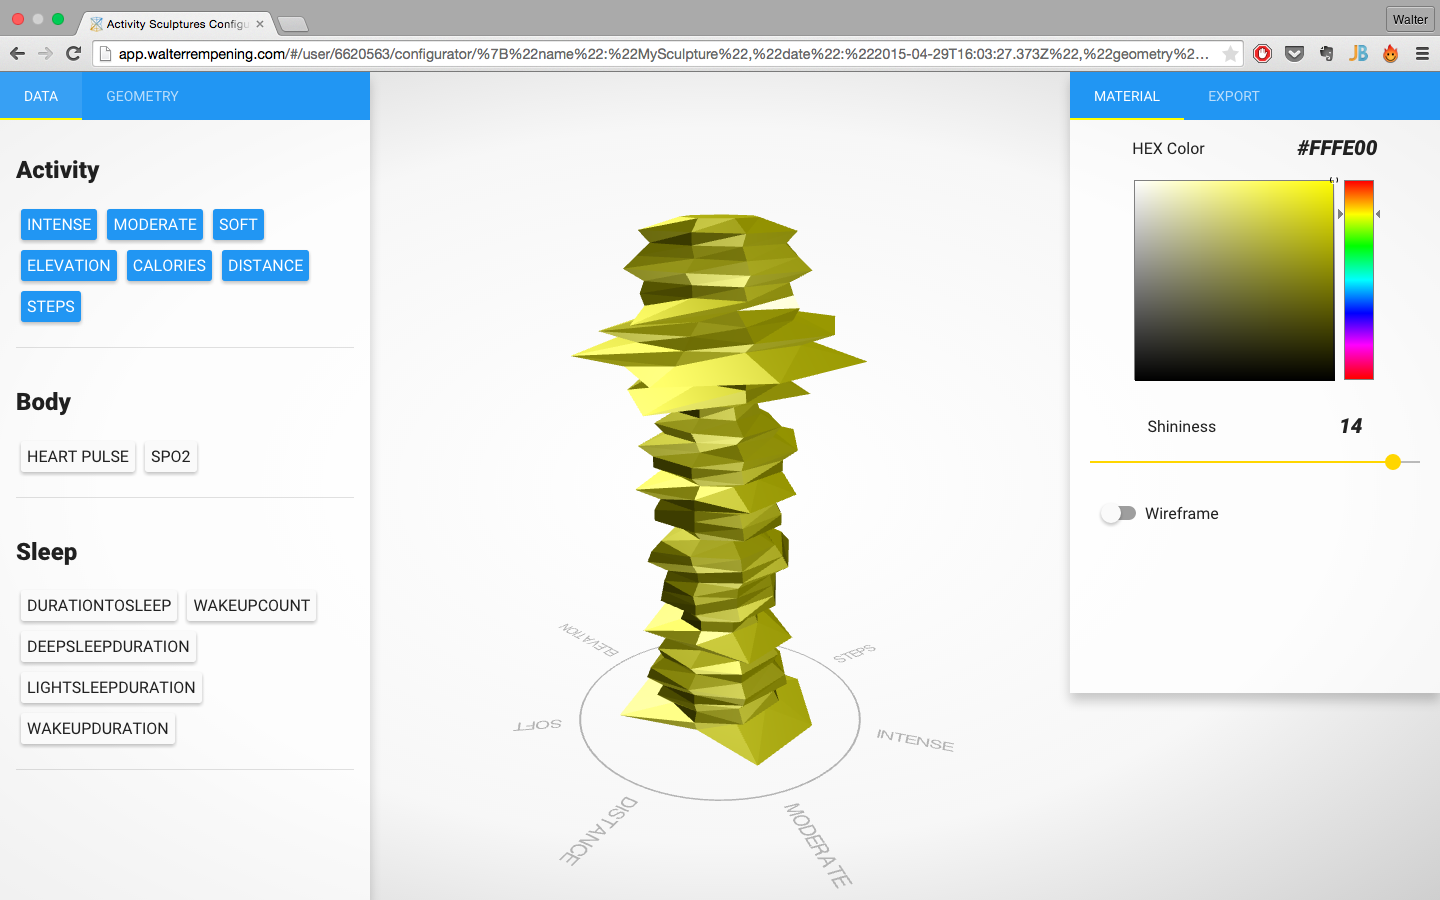
\includegraphics[width=\linewidth]{Configurator/img/configurator-ui_1}
	\caption{Data and material tabs active}
	\label{fig:configui1}
\end{minipage}
\begin{minipage}{0.45\textwidth}
\centering
  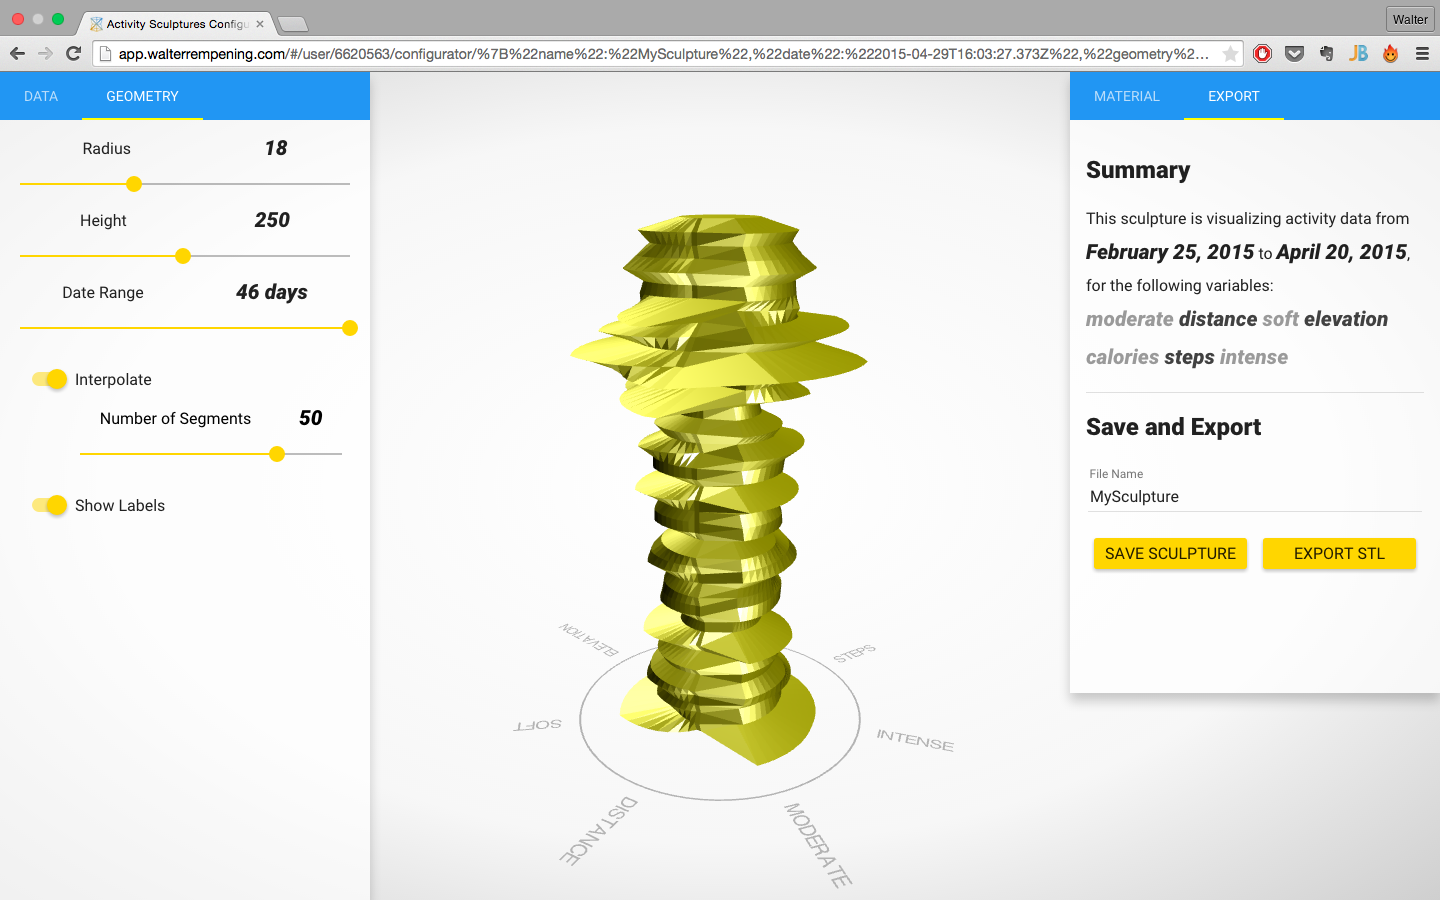
\includegraphics[width=\linewidth]{Configurator/img/configurator-ui_2}
  \caption{Geometry and export tabs active}
  \label{fig:configui2}
\end{minipage}
\end{figure}


\begin{lstlisting}[style=htmlcssjs, caption={Example of bidirectional data binding in AngularJS},label=list:ui-binding]
<!-- controller-view.html -->
<div ng-controller="PanelController as pctrl">
	<!-- ... -->
	<div flex="10" layout="row" layout-align="space-around center">
    	<span class="slider-name">Date Range</span>
		<span class="slider-value">{{ pctrl.uiGeoParams.heightSegments }} days</span>
  </div>
	<md-slider flex
		min="{{ pctrl.sliderParams.heightSegments.min }}"
		max="{{ pctrl.sliderParams.heightSegments.max }}"
		ng-model='pctrl.uiGeoParams.heightSegments'
		ng-change="pctrl.onUiParamsChange()" >
	</md-slider>
	<!-- ... -->
</div>
\end{lstlisting}

For updating the sculpture every time the user changes a parameter all widgets call the ``onUiParamsChange()'' method through the ng-change angular directive in line 12 of listing \ref{list:ui-binding}, which listens for input events. Listing \ref{list:ui-binding-ctrl} shows an excerpt of the controller's code where the slider parameter object is defined and the ``onUiParamsChange()'' method is called. This code example shows how easily is to bind controller's data into the view, not only for displaying or synchronization purposes but the controller's fields can also be used to set constrains and other attributes for UI-controls. The PanelCotnroller's code in listing \ref{list:ui-binding-ctrl} also exemplifies how other services can be injected to the controller. On lines 2 through 4 the controller injects the \textit{ModelService} from the \textit{wcModel} module. On line 15 the controller calls the ``updateMesh'' method from the \textit{ModelService}. 

\begin{lstlisting}[style=htmlcssjs, caption={Binded controller data and the called controller function from the view},label=list:ui-binding-ctrl]
// PanelController.js
var controlls = angular.module( 'wcControlls', [] );
controlls.controller( 'PanelController', 
	['ModelService', function ( ModelService ) {
	// Configuration object 
	this.sliderParams = {
	    heightSegments: {
	    	min: 1,
	        max: $scope.data.values.length - 1
	    },    
	// definition of more fields...        	
	}
    
	this.onUiParamsChange = function () {
		ModelService.updateMesh( this.uiGeoParams, this.uiMatParams );
	};
}]);	
\end{lstlisting}

The implementation of the ``updateMesh()'' method is described in listing \ref{list:ui-binding-service}. The ``updateMesh()'' method requires two objects containing geometry and material parameters which are then passed to the \textit{WCVaseGeometry} class in the ``makeSculpture()'' method on line 11 for updating the sculpture. This is achieved by looking in the \textit{SceneService} for the old sculpture removing it, creating a new one and adding it to the scene object again (see lines 7 through 12). The \textit{ModelService} exemplifies how Angular encourages strong concern separation through the use of services and modules that can be injected to controllers and services across the whole application taking advantage of reusing code as much as possible. 

\begin{lstlisting}[style=htmlcssjs, caption={Sculpture update function},label=list:ui-binding-service]
// wcModel.js
var model = angular.module( 'wcModel', [] )
model.service( 'ModelService',
	['SceneService', function ( SceneService ) {

	this.updateMesh = function ( geoArgs, matArgs ) {
	    var oldSculpture = SceneService.scene.getObjectByName( 'vase' );
	    if ( oldSculpture !== undefined ) {
	    	SceneService.scene.remove( oldSculpture );
	    }
	    sculpture = makeSculpture( geoArgs, matArgs );
	    SceneService.scene.add( sculpture );
	};
}]);
\end{lstlisting}

The configurator is an example of how the use of SPA frameworks like AngularJS are a suitable option for the implementation of highly interactive web applications that integrate well with other libraries like Threejs or D3js. As a side note, due to space constraints and the high complexity of the code base, the source code showed in this chapter was simplified for explanation purposes. For the full source code refer to the appendix \ref{app:source:repository}. 

\subsection{Backend}
The backend of the activity sculpture configurator serves as a web service from which the configurator's front end queries user data that is processed by the web server through the Withings API and some data manipulation modules. The following section attempts to explain how the Withings API integrates with other parts of the web server and the subsequently data manipulation tasks performed. 

\subsubsection{Withings API Integration}
\label{sub:ApiIntegration}
The Withings API is used to complete to tasks: user authentication and data import. In order to have access to user's data from third party applications as the configurator, users have to give these applications their approval. The Withings API implements authentication through the \textit{OAuth} 1.0 protocol. \textit{OAuth} is an open standard that provides a process for authorization of third-party applications to server resources or for clients to access server resources using credentials of other web services\cite{hammer2010oauth}. \textit{OAuth} is commonly used in web services where users may login in using their twitter, facebook or google account. The process of authentication is performed through several HTTP calls. The Withings API requires third party developers to create a developer account and register the application. Every application is assigned an API key and secret. These keys are needed for the \textit{OAuth} process as they are have to be present in every HTTP call. The authentication process involves 3 steps. For the Withings API developers first request an end-user token, a successful response from the API provides an oauth token and oauth token secret. With the received tokens developers redirect users to web site where they can login with their credentials and authorize the third-party application the use of their data. If the authorization was granted the developer receives an oauth token and the user id. The final step consists in requesting a user data access token which once received allows third party applications to access data for the specified user. 

In order to simplify the process of generation the URLs for the HTTP calls in the \textit{OAuth} authentication process the web configurator makes use of the \textit{Passport}\cite{passport} framework which supports different authentication methods and also provides session handling. Being also written in JavaScript the framework integrates seamlessly with the backend's Node.js and Express architecture. Through the use of the \textit{Passport} frame work the whole \textit{OAuth} authentication process is reduced to only to two API calls (see listing \ref{list:auth}). The first API call (lines 2 through 5) defines the address the client calls when login in to the configurator. \textit{Passport} uses preconfigured API Keys from and Withings developers account and starts the token interchange process. After clicking the login button the user will be redirected to a Withings website where his credentials are required. After he has granted permission to the configurator to access his data he will be redirected to a predefined callback URL address which is the configruator's webserver's second API call (lines 7 through 13 of listing) that will store the received user data access tokens in a cookie and redirects the user to the Angular frontend. 

\begin{lstlisting}[style=htmlcssjs, caption={Passport OAuth authentication implementation},label=list:auth]
// routes.js
app.get('/auth/withings', passport.authenticate('withings'),
    function(req, res, next) {
      console.log("Withings OAuth flow started");
});

app.get('/auth/withings/callback', passport.authenticate('withings',
	{failureRedirect: '/' }),
	function(req, res, next) {
	  res.cookie('user', JSON.stringify(req.user), {maxAge: 2592000000});
	  res.redirect('/#/user/' + req.user.id);
	}
);
\end{lstlisting}
After this point the configurator's backend is able to request user's data through the Withings API. The Withings API provides access to all measured information about the user being it activity, body and sleep measures, which can be requested for a single date or for a date range from up to 200 days. As an example listing \ref{list:apireq} shows example code for a query for a single days activity data and the received data in a JSON object. Every Withings API request URL has to contain a series of parameters like the oauth consumer key, signature, token and others, which makes the generation of the requests quite cumbersome. To address this issue a \textit{Passport} extension module called \textbf{Withings-API}\cite{withingsApi} was used. This module abstracts the generation of request URLs to a JavaScript object making it a comfortable way of managing API calls. 

\begin{lstlisting}[style=htmlcssjs, caption={Withings API query and response example},label=list:apireq,float=t]
// Request URL
https://wbsapi.withings.net/v2/measure?action=getactivity&userid=29&date=2015-05-15&more_parameters...

// API JSON response
{
   "status": 0,
   "body": {
       "date":"2015-05-15",
       "steps":6523,
       "distance":4600,
       "calories":408.52
       "elevation":18.2,
       "soft": 5880,
       "moderate": 1080,
       "intense": 540, 
       "timezone":"Europe/Berlin"
    }
}
\end{lstlisting}

\subsubsection{Data Processing}
The JSON objects in which the Withings API packs the response data integrate well with the configurator's architecture because \textit{MongoDB} works seamlessly with JSON objects allowing for direct storage of the received data. The requests performed by the configurator's backend ask always for several days worth of data and unfortunately the received JSON object contains the data not ordered by date but in semi random order. Before storing the data to the database a sorting algorithm is performed on the data and stored ordered by date. 

The configurator visualizes the activity data in the charts displayed in the dashboard section and in the activity sculpture in the configurator section. Due that the data visualization in both sections is performed by different frameworks namely D3js and Threejs respectively, each require the data in a unique format. Because the visualizations are rendered by the frontend the formatting and processing of the data is performed by the api module consisting of the \textit{wcUserData} service and a utility class for data transformations called \textit{wcDataUtils}. The \textit{wcUserData} stores a User object that contains all the activity data, stored sculptures for the user and the system settings configured by the user. For other controllers to gain access to the data, they only have to include this service and depending on the visualization to be performed the \textit{wcDataUtils} class contains formatting methods that return the data with the correct format for the needed visualization type. 

\subsection{Challenges}
The activity sculpture configurator is an application comprised of many software elements with different purposes which makes it not an easy task integrating these parts in an harmoniously manner. In retrospective the main challenge was to estimate the time needed to develop the configurator. At the beginning of the development the author had planned a 3 week time span for completely implementing the configurator which was very inaccurate as the complexity of the functionality was underestimated. At the end the development time was prolonged to two months. Around 5 weeks were spend developing the backend and around 3 weeks were used for the frontend. It is important to note that during the research phase of this work, the author had already prepared a deployment server from which the configurator would be available to the public. Due to the high requirements the software had to be developed in a very abstract and dynamic approach as it had to adapt a variety of users. 

Working with the Withings API and the Pulse Ox tracker was at times somewhat frustrating and limiting as during the development both showed some stark pitfalls. The Pulse Ox does not measure heart-rate and SPO2 automatically requiring users to take the sensor from the wristband and perform the measurements manually. Another annoying detail is that for measuring sleep activity the fitness tracker has to be also set on sleep monitoring mode and for best results it had to be worn almost 24/7 which at the long rung showed to be annoying. The Whitings API's documentation did not provide enough information in the documentation some times it was vague. Unfortunately in the web there are not many resources available for guidance. The semi randomly ordered data objects was also an added work load. The implementation of session handling functionality as it was not planned at first but was found to be needed during the development phase. Due to time constrains only a working implementation was possible. 

With the fully working activity sculpture configurator, the test phase of the developed concepts took place. The next chapter provides in depth information about the considerations made for the user study and findings gained. 


\end{document}